\section{Background}
\vspace{-0.5cm}
\subsection{Microneedles as Biosensors}
\vspace{-0.5cm}
For continuous monitoring, electrochemical MN biosensors are used, which consist of a signal transducer (the MN) coated with a recognition element that forms specific interactions with the target biomarker transmitting a quantifiable electrical signal that correlates with target’s concentration.
\begin{center}
    \begin{figure}[H]
    \centering
    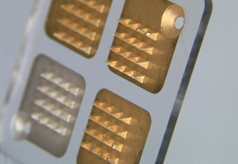
\includegraphics[width=.4\textwidth]{img/microneedle_patch.png}
    \caption{Example Image of a Microneedle array for real-time, minimally invasive drug monitoring of phenoxymethylpenicillin \cite{rawson2019microneedle}}
    \label{fig:microneedle}
\end{figure}
\end{center}
\vspace{-1cm}
Our MN biosensor has two main application purposes: (1) accessing the ISF by penetrating the stratum corneum into the viable epidermis and (2) acting as a platform for the recognition element. Hence, more holistic theoretical research has been performed on skin structure and MN design considerations for translation to in-vivo testing in \autoref{Appendix_A} and \autoref{micro_no2}.
\subsection{Nitrite Investigations}
Nitrite has been measured at higher levels in septic patients vs healthy patients (52.8$\pm$44.0 vs 29.6 $\pm$8.9 $\mu$M)\cite{pmid12688539} and performs better as a biomarker for diagnosing septic shock than other biomarkers such as procalcitonin and C-reactive protein. (Positive predictive value (PPV):0.96) \cite{pmid9142024}.\\\\
We aim to measure nitrite concentrations ranging from healthy to septic levels \cite{pmid12688539} in solution by performing differential pulse voltammetry, obtaining a calibration curve, examining the oxidation of nitrite (NO$_{2}^{-}$) to nitrate (NO$_{3}^{-}$), shown in \autoref{eqn:nitriteredox1} and \autoref{eqn:nitriteredox2}.
\begin{align} \label{eqn:nitriteredox1}
   NO\textsubscript{2}\textsuperscript{-} \ \xrightleftharpoons{}  NO\textsubscript{2} \ + \  e\textsuperscript{-}
\end{align} 
\begin{align}\label{eqn:nitriteredox2}
  2NO\textsubscript{2} \ + \ H\textsubscript{2}O \xrightarrow{}\  2H\textsuperscript{+} \ + \ NO\textsubscript{2}\textsuperscript{-} \ + \  NO\textsubscript{3}\textsuperscript{-}
\end{align}
Differential pulse voltammetry (DPV) measures the concentration of electrolytes in solution by applying a potential (E) at the working electrode (WE) and reference electrode (RE). The counter electrode (CE) provides a route for current to flow. A series of pulses of increasing steps is applied to the WE and the difference in current between steps is measured \cite{D1CP00661D}. A calibration curve is then constructed from the peaks of the curve. \\\\
Experiments utilising disposable gold electrodes, where the WE, RE and CE are all located on a 10x8mm polycarbonate surface, were then performed. These electrodes have a good electrochemical response, as well as being cheap and disposable, favouring use in a clinical setting as a biosensor \cite{FERRARIO201236}.\\\\
Human blood contains around 33–52g/L of albumin. Evidence shows that albumin's presence interferes with electrode activity. \cite{doi:10.1177/000456329102800111}.
%======================================================================================================
\subsection{Hydrogen Peroxide Investigations}
Hydrogen peroxide, H\textsubscript{2}O\textsubscript{2}, is a chemical that is commonly found in multiple biological processes \cite{Pravda2014}. It is reported that a drastic increase in \textit{in-vivo} hydrogen peroxide concentration is usually accompanied by systemic inflammations. Previous research observed an approximate 10-fold increase in hydrogen peroxide concentration, from 21-36$\mu$M in blood from healthy individuals \cite{FORMAN201648}, to 316$\pm$242.8$\mu$M in septic blood \cite{VanAsbeck1995}. Therefore, hydrogen peroxide is a novel sepsis biomarker and is highly suitable for clinical continuous-monitoring techniques. Its capability to identify sepsis and indicate the severity of infection is significant for sepsis diagnosis, evolution evaluation and prognosis prediction.\\\\
\noindent{A strategy based on reduction-oxidation reactions between hydrogen peroxide and Prussian blue (PB) is proposed by Chen \textit{et al.} \cite{C9AN02438G} is used to detect the presence of hydrogen peroxide. Prussian blue demonstrates an outstanding hydrogen peroxide sensing range with low operating potential. This two-step reaction commences by reducing Prussian blue to Prussian white (PW) (shown in \autoref{eqn:h2o2redox1}) where hydrogen peroxide is further reduced to water (shown in \autoref{eqn:h2o2redox2}).}
\begin{align} \label{eqn:h2o2redox1}
    KFe^{3+}[Fe\textsuperscript{2+}(CN)\textsubscript{6}]\textsuperscript{4-} \ + \ & K\textsuperscript{+} \ + \   e\textsuperscript{-} \ \xrightleftharpoons{} \\ \nonumber & K\textsubscript{2}Fe\textsuperscript{2+}[Fe\textsuperscript{2+}(CN)\textsubscript{6}]\textsuperscript{4-}
\end{align}
\begin{align} \label{eqn:h2o2redox2}
    & 2K\textsubscript{2}Fe\textsuperscript{2+}[Fe\textsuperscript{2+}(CN)\textsubscript{6}]\textsuperscript{4-} \ + \  H\textsubscript{2}O\textsubscript{2} \ + \ 2H\textsuperscript{+} \ \xrightleftharpoons{} \\ \nonumber & \quad \quad 2K\textsubscript{2}Fe\textsuperscript{3+}[Fe\textsuperscript{2+}(CN)\textsubscript{6}]\textsuperscript{4-} \ + 2H\textsubscript{2}O \ + \ 2K\textsuperscript{+}
\end{align}
\begin{figure}[H]
    \centering
    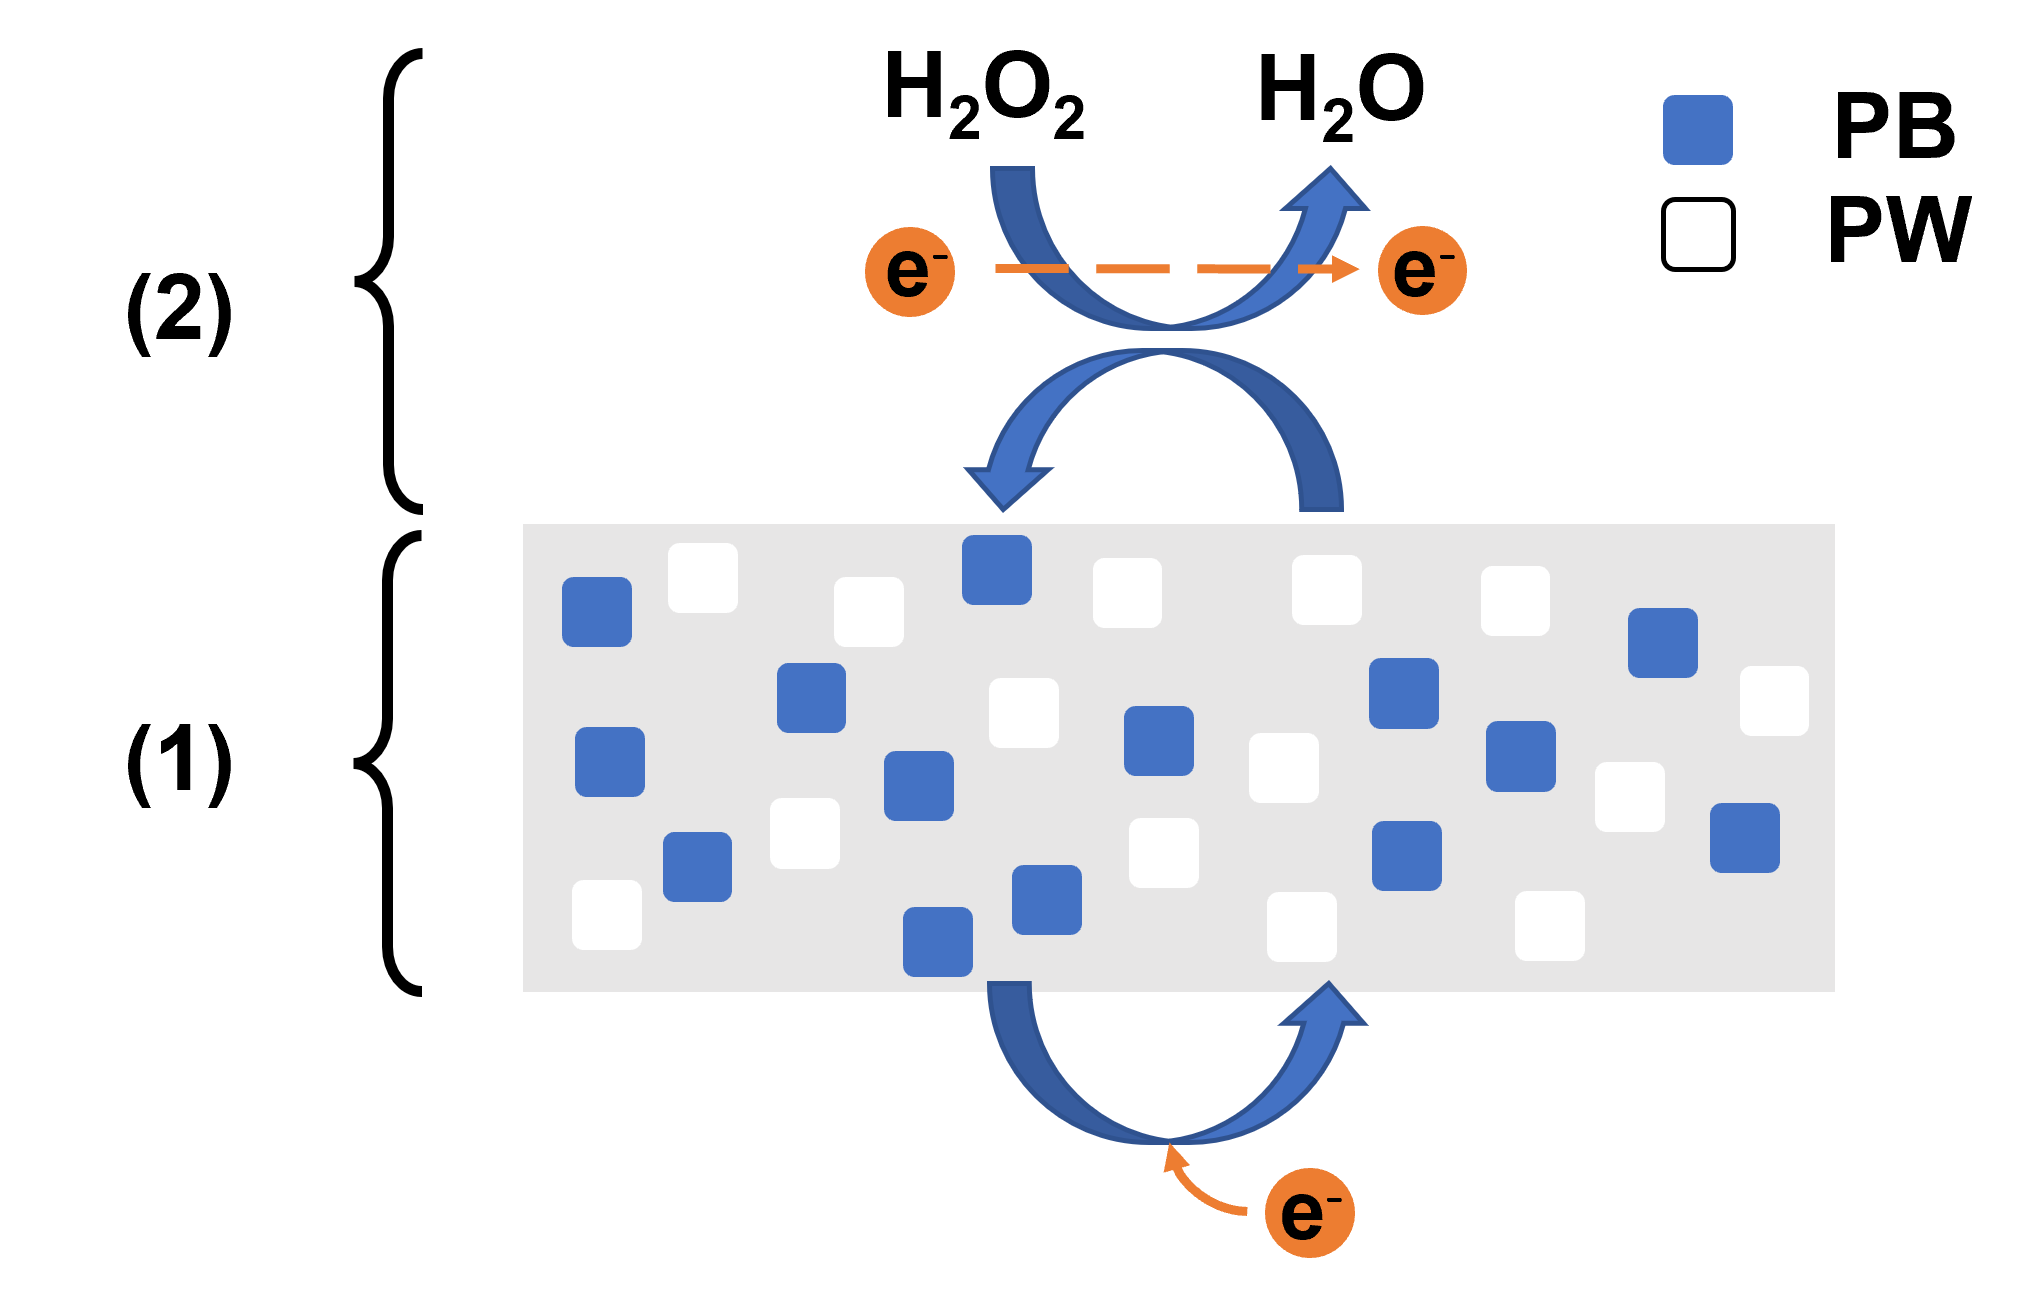
\includegraphics[width=.4\textwidth]{img/pb_h2o2.png}
    \caption{Reaction between hydrogen peroxide and Prussian blue.}
    \label{fig:pb_h2o2}
\end{figure}
%======================================================================================================
\subsection{Lactate Investigations}
Patients suffering from sepsis often develop Sepsis-Associated Hyperlactatemia (SAHL). Multiple proposed theories can explain SAHL. One possible hypothesis suggests the cause of SAHL is the increase of aerobic glycolysis rates after adrenergic stimulation \cite{garcia2014sepsis}.
Hyperlacatatemia can be characterised by a serum concentration exceeding 4mM; However,  other literature suggests lower thresholds beginning at 3mM can also indicate a significant septic state \cite{singer2014ed}.
Real-time monitoring of lactate levels in clinical settings is vital in ensuring a sharp increase in levels exceeding healthy patients can be detected quickly. This allows antibiotic administration or other appropriate measures to be taken before a fatal state is reached \cite{gyawali2019sepsis}.
Since lactate cannot directly engage in any redox reaction with the gold electrode, our sensor requires the use of enzymes such as lactate oxidase (LOX), which can be drop coated onto the surface of our electrode in a hydrogel matrix. The LOX can then oxidise lactate in the presence of oxygen to produce pyruvate and hydrogen peroxide. The gold electrode can then detect the peroxide.
\begin{align}
    Lactate + O_{2}  \xrightarrow{} Pyruvate + H_{2}O_{2}
\end{align}
\begin{align}
    H_{2}O_{2} + O_{2}  \xrightarrow{} 2e^{-}+2H^{+}
\end{align}
In this project, we develop enzyme-based electrodes that can detect lactate levels of both healthy and septic patients in the 0.0-4.5mM range.
\subsection{Statistics of Diagnosis}
When working with different sepsis biomarkers, readings must be specific and predictive. Particularly in the case of sepsis, treatment includes the administration of antibiotics. If antibiotics are delivered unnecessarily, it could lead to antibiotic resistance.\\\\
To evaluate the success of a  diagnostic technique, the sensitivity, specificity and predictive values are commonly used by clinicians. The biomarker must be assessed for both false and true results against a pre-established gold standard diagnosis (assumed 0 false positives) to calculate each of these variables.\\\\
The calculations for these statistics can be seen in \autoref{fig:statistics}
\cite{christenson2007evidence}.
\begin{figure}[h]
    \centering
    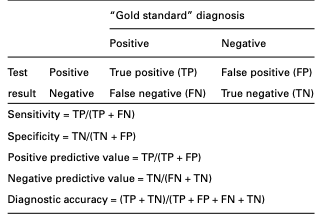
\includegraphics[width=0.5\textwidth]{img/statistics of diagnosis.png}
    \caption{Statistics of diagnosis \cite{christenson2007evidence}}
    \label{fig:statistics}
\end{figure}
For both predictive values and overall diagnostic accuracy, variations occur with the prevalence of sepsis. PPV can increase dramatically with increased prevalence, so sensitivity and specificity are often more frequently used to describe the efficacy of detection methods.  However, these are not immune to variability, especially in sepsis, which is not binary.  Patients exhibit rising levels of biomarkers before actually becoming septic. In such cases, a ‘cut off mark’ is not always a singular number but more often a range \cite{xia2013translational}. \\\\
A more useful and less discriminatory way of quantifying usefulness is looking at the relationship between sensitivity and specificity by plotting Receiver Operating Characteristics (ROC). Where there exists a range of values rather than a single cutoff value, sensitivity and specificity value pairs can be determined for different levels of biomarker concentration. We can obtain a ROC curve by plotting 1-specificity (false positive rate) versus sensitivity. The symmetry of the graph and the area under it can be used to convey diagnostic accuracy, allowing clinicians to utilise sensor readings \cite{kampfrath2013brief}. 
\subsection{Aptamer-Based Biosensors}
Nucleic acid aptamers are smaller in size, more chemically stable and cost-effective as biorecognition elements than enzymes or antibodies \cite{song2008aptamer}. Aptamers can be isolated from a library of sequences via Systematic Evolution of Ligands by Exponential Enrichment (SELEX) and can selectively bind to many different types of small molecules such as biomarkers, metal ions, antibiotics and more \cite{cai2018investigations}. Aptamers can undergo different conformational changes upon target binding to form structural shapes such as hairpins, bulges, and G-quadruplexes \cite{riccitelli2010computational}; this results in a change in distance between the modified redox group and electrode surface, thus, leading to a change in the current.\\\\
Interrogating of aptamer-based biosensors using chronoamperometric detection offers drift resistance and subsecond temporal measurements of target molecules \textit{in-situ}. In Plaxco's analysis of current transient lifetime, the initial rapid exponential phase due to the electrode double layer charging is ignored, and the lifetime of the slower faradic current decay (due to the electron transfer of the methylene-blue) is measured. Experimental results using Tobramycin show a five times reduction in decay lifetime from no target to a saturated target concentration. The authors predicted linear variation of exponential decay phase (corresponding to a single-exponential fit) with target concentration. They claimed similar lifetimes for the two aptamer states, stating difficulty in extracting relevant amplitudes with sufficient precision. Multiexponential decomposition was not used to justify the electron transfer rates proximity but resorted to approximate current decay lifetimes using monoexponential fit. The derivation for the multiexponential current output of aptamer-based biosensors was interrogated using chronoamperometry (\autoref{Aptamer_multiexp}).\\\\
Multiexponential decomposition is an ill-posed problem, particularly with signals with intrinsic noise \cite{jibia2012appraisal}. In this project, we present an accurate and representative model for analysing chronoamperometric detection in aptamer biosensors from the first principles, considering the physical nature of DNA motion \cite{ouldridge2012coarse}. Combining this with the chronoamperometric signal by decomposing the general multiexponential signal using a NIL method  \cite{provencher1982contin}, we extract the bound and unbound aptamer rate constants and their respective concentrations.\\\\


